\tikzset{
	visible on/.code={%
		\ifthenelse{\equal{#1}{}}{%
			\tikzset{alt={<\value{beamerpauses}->{}{opacity=0}}}%
		}{%
			\tikzset{alt={#1{}{opacity=0}}}%
		}%
	},%
	alt/.code args={<#1>#2#3}{%
		\alt<#1>{\pgfkeysalso{#2}}{\pgfkeysalso{#3}}%
	}%
}

\definecolor{red}{HTML}{972e21}
\definecolor{yellow}{HTML}{ebb83f}
\definecolor{blue}{HTML}{7999db}

\begin{frame}
  \frametitle{\problemtitle}
  \begin{block}{Problem}
  	Given $n$ points in the plane, determine if $k=3$ lines are sufficient to cover all points.
  \end{block}
  \begin{center}
  	%37-unique | solution is not unique...
  	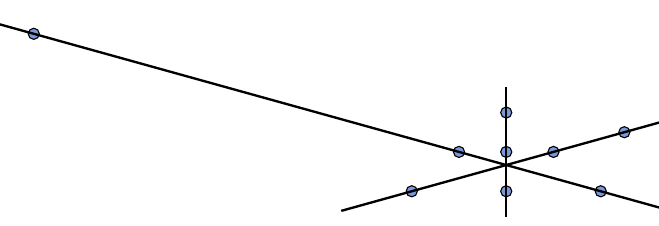
\begin{tikzpicture}[x=0.3cm,y=-0.25cm,every node/.style={circle,draw,fill=blue,inner sep=0.05cm,outer sep=0cm}]
  		\node at (6,5) (a) {};
  		\node at (6,7) (b) {};
  		\node at (6,9) (c) {};
  		\node at (8,7) (d) {};
  		\node at (10,9) (e) {};
  		\node at (4,7) (f) {};
  		\node at (2,9) (g) {};
  		\node at (11,6) (h) {};
  		\node at (-14,1) (i) {};  		
  		\draw[visible on=<2->,shorten <= -1cm,shorten >= -1cm, line width=0.03cm] (e) -- (i);
  		\draw[visible on=<3->,shorten <= -1cm,shorten >= -1cm, line width=0.03cm] (g) -- (h);
  		\draw[visible on=<4->,shorten <= -0.4cm,shorten >= -0.4cm, line width=0.03cm] (c) -- (a);
  	\end{tikzpicture}
  \end{center}
  \pause[5]
  \begin{block}{Solution}
  	\begin{itemize}
  		\item If we have at most $k$ points the answer is obviously Yes.
  		\item If we select $k+1$ points, one line has to go through two of those points.
  		\pause
			\item Given $k$ and $n > k$ points solve the problem recursively:
  		\begin{itemize}
  			\item Select $k+1$ points and try all lines through two points.
  			\item For each line remove all covered points.
  			\item Check recursively with $k-1$ and the remaining points.
  		\end{itemize}
  		\pause
			\item Time complexity for ($k=3$): $n\cdot\prod_{i=1}^{k}\binom{i+1}{2}=18\cdot n$
  	\end{itemize}
  \end{block}
\end{frame}

\begin{frame}
	\frametitle{\problemtitle}
	\begin{block}{More Observations}
		\begin{itemize}
			\item There must be a line which covers at least \alert{a third} of all points.
			\pause
			\item There must be a line which covers at least \alert{half} of all remaining points.
			\pause
			\item There must be a line which covers \alert{all} remaining points.
		\end{itemize}
	\end{block}
	\pause
	\begin{block}{Solution 2}
		\begin{itemize}
			\item Recursively select a random line through two points.
			\item At step $k$ check if the chosen line covers $\frac{1}{k}$ of all points.
			\pause
			\begin{itemize}
				\item[Yes:] recursively continue with $k-1$ and the remaining points.
				\pause
				\item[No:] try another line or abort after sufficient many tries \textcolor{gray}{($\sim 5\cdot k$)}.
			\end{itemize}
			\pause
			\item Time complexity for ($k=3$): $n\cdot5\cdot k!=30\cdot n$
		\end{itemize}
	\end{block}
\end{frame}




%\begin{frame}
%	\frametitle{\problemtitle}
%	\begin{center}		
%		\begin{tikzpicture}[x=0.42cm,y=0.37cm,line width=0.05cm]
%			\draw (0,0) rectangle(7,10);
%			
%			\draw[fill=red] (0,2) rectangle(1,3);
%			\draw[fill=red] (0,1) rectangle(2,2);
%			\draw[fill=red] (0,0) rectangle(1,1);
%			\draw[fill=red] (1,0) rectangle(3,1);
%			
%			\draw[fill=red] (3,0) rectangle(5,1);
%			\draw[fill=red] (4,1) rectangle(5,2);
%			\draw[fill=red] (4,2) rectangle(5,3);
%			\draw[fill=red] (4,3) rectangle(5,4);
%			\draw[fill=red] (5,0) rectangle(7,1);		
%			\draw[fill=red] (6,1) rectangle(7,2);
%			
%			
%			\draw[fill=blue,visible on=<2->] (0,3) rectangle(1,5);
%			\draw[fill=blue,visible on=<2->] (0,5) rectangle(1,7);
%			\draw[fill=blue,visible on=<2->] (0,7) rectangle(1,9);
%			\draw[fill=blue,visible on=<3->] (0,9) rectangle(2,10);
%			
%			
%			\draw[fill=blue,visible on=<4->] (1,2) rectangle(2,4);
%			\draw[fill=blue,visible on=<4->] (1,4) rectangle(2,6);
%			\draw[fill=blue,visible on=<4->] (1,6) rectangle(2,8);
%			\draw[fill=blue,visible on=<5->] (1,8) rectangle(3,9);
%			
%			
%			\draw[fill=blue,visible on=<6->] (2,1) rectangle(3,3);
%			\draw[fill=blue,visible on=<6->] (2,3) rectangle(3,5);
%			\draw[fill=blue,visible on=<6->] (2,5) rectangle(3,7);
%			\draw[fill=blue,visible on=<7->] (2,7) rectangle(4,8);
%			\draw[fill=blue,visible on=<7->] (2,9) rectangle(4,10);
%			
%			
%			\draw[fill=blue,visible on=<8->] (3,1) rectangle(4,3);
%			\draw[fill=blue,visible on=<8->] (3,3) rectangle(4,5);
%			\draw[fill=blue,visible on=<8->] (3,5) rectangle(4,7);
%			\draw[fill=blue,visible on=<9->] (3,8) rectangle(5,9);
%			
%			
%			\draw[fill=blue,visible on=<10->] (4,4) rectangle(5,6);
%			\draw[fill=blue,visible on=<10->] (4,6) rectangle(5,8);
%			\draw[fill=blue,visible on=<11->] (4,9) rectangle(6,10);
%			
%			
%			\draw[fill=blue,visible on=<12->] (5,1) rectangle(6,3);
%			\draw[fill=blue,visible on=<12->] (5,3) rectangle(6,5);
%			\draw[fill=blue,visible on=<12->] (5,5) rectangle(6,7);
%			\draw[fill=blue,visible on=<12->] (5,7) rectangle(6,9);
%			
%			
%			\draw[fill=blue,visible on=<13->] (6,2) rectangle(7,4);
%			\draw[fill=blue,visible on=<13->] (6,4) rectangle(7,6);
%			\draw[fill=blue,visible on=<13->] (6,6) rectangle(7,8);
%			\draw[fill=blue,visible on=<13->] (6,8) rectangle(7,10);
%		\end{tikzpicture}
%	\end{center}
%	\begin{block}{Solution}
%		\begin{itemize}
%			\item There is an greedy strategie which finds a perefect matching should it exists
%			\pause
%			\begin{itemize}
%				\item Go from left to right
%				\item Place as many $1\times 2$ blocks from botton to top as you can fit in the current column
%				\item If needed place $2\times 1$ blocks on top which go into the next column 
%			\end{itemize}
%			\pause[14]
%			\item To simulate this efficiently we only to store the height of the lowest brick comming from the left%
%			\item This value either increases or decreases by $1$ if we go to the next column
%		\end{itemize}
%	\end{block}
%\end{frame}
